\subsection{Definiciones}

Sea G=(V,E) un grafo simple:

\begin{itemize}
\item Definición 1: D $\subseteq$ V es un \textbf{conjunto dominante} (CD) $\iff$ $\forall$ v $\in$ V, v $\in$ D ó $\exists$ w $\in$ D tal que (v,w) $\in$ E (tiene un vecino en D).
\item Definición 2: D $\subseteq$ V es un \textbf{conjunto independiente} (CI) $\iff$ $\forall$ v,w $\in$ D, (v,w) $\not\in$ E.
\item Definición 3: D $\subseteq$ V es un \textbf{conjunto independiente dominante} (CID) $\iff$ D es dominante e independiente.
\item Definición 4: D $\subseteq$ V es un \textbf{conjunto independiente dominante mínimo} (CIDM) $\iff$ D es el conjunto independiente dominante de V con menos nodos. Es decir que $\forall$ D' $\subseteq$ V tal que D' es independiente dominante, \#(D) $\leq$ \#(D').
\item Definición 5: D $\subseteq$ V es un \textbf{conjunto independiente maximal} (CIMax) $\iff$ D es independiente y $\not\exists$ D' $\subseteq$ V independiente tal que D $\subset$ D' ($\subset$ estricto).
\end{itemize}

\subsection{Ejercicio A}

\textit{Relacionar el problema de CIDM con el problema 3 del TP 1 (i.e., similitudes y diferencias):}

\medskip

Si definimos a G=(V,E) grafo simple para que represente al tablero de ajedrez que se forma en el ejercicio 3 del tp1, los nodos serían una cuadricula de la pinta (sin considerar los ejes, eso lo hacemos después):

\begin{figure}[h]
\begin{center}
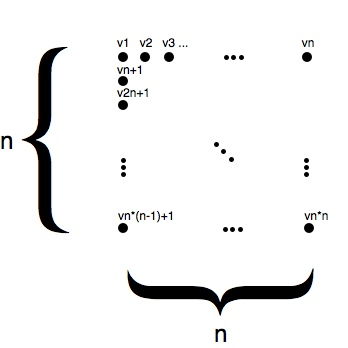
\includegraphics[scale=0.5]{imagenes/grafos-ej1-tp3-1.jpg}
\end{center}
\end{figure}

Donde 'n' es el parámetro del ejercicio que indica el tamaño de lado del tablero.

\newpage

Ahora, como el ejercicio consiste en poner la \underline{mínima} cantidad de \underline{caballos} para que todas las casillas tengan un caballo o bien estén amenazadas, podemos representar las 'amenazas' como los ejes del grafo, por ejemplo:

\begin{figure}[h]
\begin{center}
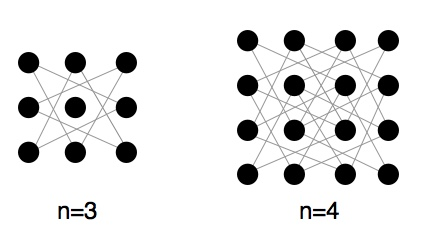
\includegraphics[scale=0.5]{imagenes/grafos-ej1-tp3-2.jpg}
\end{center}
\end{figure}

\textit{Observación: como cualquier posición x que amenaza a otra posicion 'y' sería amenazada si pongo un caballo en 'y', podemos representar el problema con un grafo simple y no un digrafo.}

\medskip

Entonces los ejercicios son similares ya que lo que estamos buscando en el ejercicio del TP1 es la mínima cantidad de caballos para que todas las posiciones (nodos) tengan un caballo o esten amenazadas (dominadas).

Es decir, si los caballos son un conjunto D de vértices en V, queremos hallar \#(D) tal que:
\begin{itemize}
\item $\forall$ v $\in$ V, v $\in$ D o $\exists$ w $\in$ D tal que (v,w) $\in$ E $\iff$ D es dominante.
\item $\forall$ D' $\subseteq$ V tal que D' es dominante, \#(D) $\leq$ \#(D') $\iff$ D es mínimo entre los conjuntos dominantes de V.
\end{itemize}

Por lo tanto el problema consiste en hallar un conjunto dominante mínimo pero, a diferencia del problema en este TP, puede o no ser independiente.
Esto se debe a que existen respuestas para el problema del TP1 donde hay caballos en ciertas posiciones que se amenazan entre sí:

\begin{figure}[h]
\begin{center}
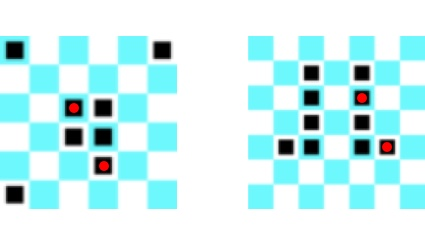
\includegraphics[scale=0.5]{imagenes/grafos-ej1-tp3-3.jpg}
\end{center}
\end{figure}

\textit{Observación: estos graficos fueron extraidos de la página: http://home.earthlink.net/~morgenstern/solution/knsols1.htm. El primero representa una solución óptima del ejercicio del TP1 con un tablero de 6x6 y la segunda imágen es para un tablero de 7x7. En ambas, se marcan con un punto negro los casilleros que tienen un caballo y, como vemos señalado en rojo, hay caballos en posiciones que se amenazan entre sí.}

\medskip

Mas alla de eso, ambos problemas son de optimización combinatoria. Los conjuntos factibles son los vertices de un grafo que cumplen ciertas condiciones (si bien como dijimos antes, no son las mismas para los dos problemas) y la función de optimalidad consiste en minimizar la cantidad de vértices del conjunto.

\newpage

\subsection{Ejercicio B}

\textit{Demostrar que todo conjunto independiente maximal es un conjunto dominante:}

\medskip

Sea G=(V,E) un grafo simple y D $\subseteq$ V un conjunto independiente maximal, quiero ver que D es un conjunto dominante.\\
Supongamos (por absurdo) que D no es un conjunto dominante:
\begin{itemize}
\item[] $\Rightarrow$ $\exists$ v $\in$ V tal que v $\not\in$ D $\wedge$ $\forall$ w $\in$ D, (v,w) $\not\in$ E (no es vecino de ningún nodo en D).
\item[] $\Rightarrow$ D$\cup$\{v\} es independiente ya que como D es independiente sucede que $\forall$ w $\in$ D$\cup$\{v\} $\not\exists$ x $\in$ D tal que (x,w) $\in$ E.
\item[] $\Rightarrow$ Absurdo! pues D era maximal y $\exists$ D' = D$\cup$\{v\} tal que D' es independiente y D $\subset$ D', asi contradiciendo el hecho de que D es un conjunto independiente maximal.
\end{itemize}
Este absurdo vino de suponer que D no era dominante.\\
Por lo tanto, si D es un conjunto independiente maximal $\Rightarrow$ D es dominante.

\subsection{Ejercicio C}

\textit{Describir situaciones de la vida real que puedan modelarse utilizando CIDM:}

\medskip

\begin{itemize}
\item \textbf{El turista:} tenemos un conjunto de ciudades que forman un grafo simple conexo donde los nodos son las ciudades y dos nodos estan conectados si y solo si las ciudades son vecinas. Suponiendo que queremos conocer tantas culturas distintas como sea posible, decidimos que no queremos visitar ningun par de ciudades vecinas ya que sus culturas son muy similares. Como el problema que proponemos consiste en hallar un conjunto mínimo de ciudades (nodos en el mapa) tal que toda ciudad sea visitada o bien una ciudad vecina sea visitada pero no ambas (el conjunto de nodos sea independiente y dominante), podemos decir que estamos buscando un CIDM.
\item \textbf{Spamear una red social:} supongamos que tenemos un virus que se ocupa de spamear Facebook de manera que un mensaje sea propagado por toda la red. Asumimos que los usuarios de Facebook son nodos en un grafo simple conexo y que dos nodos estan conectados si y solo si esos dos usuarios son amigos en la red. Ahora, el virus no quiere ser descubierto, asi que lo que debe hacer es infectar la menor cantidad de cuentas que no sean amigas, ya que si spamea demasiadas cuentas o un par de cuentas que son amigas, sería mucho más fácil de descubrirlo. Luego, estamos buscando el mínimo conjunto de nodos en la red de usuarios tal que todos los usuarios vean el mensaje (dominación) y dos amigos no sean infectados a la vez (independencia), el cual es un CIDM.
\item \textbf{Cámaras de seguridad en un barrio:} tenemos casas en un barrio que representan los nodos de un grafo simple conexo, donde dos nodos estan conectados si y solo si sus casas respectivas con vecinas. Queremos poner cámaras de seguridad en el barrio de manera que toda casa tenga una cámara de seguridad o la tenga una casa vecina, ya que el rango de cobertura de la cámara es amplio y puede filmar la casa donde está y también las vecinas (dominación). No queremos poner cámaras en dos casas vecinas (independencia) para que no sea tan notorio y arruine el paisaje. A la vez, tenemos un presupuesto limitado, por lo cual queremos poner poner tan pocas cámaras como sea posible (minimalidad). Por lo tanto, el conjunto de casas que estamos buscando para ponerles cámaras es un CIDM.
\end{itemize}